%!TEX root = ..\Master.tex

\subsection{Support Vector Machines}
The support vector machine is a supervised learning algorithm. It can also be referred to as a sparse kernel machine. 
Compared to neural network, it sometimes gives a cleaner and more powerful way of learning complex non-linear functions. 
The goal of SVM is to maximise the margin between two clusters.

\subsubsection{Linear}
The standard SVM decision boundary is given by equation \ref{math:stdlin}.
\begin{equation}
\label{math:stdlin}
\textbf{w}^T\textbf{x}_{new} + b
\end{equation}
Objects lying on either side of the decision boundary will be classified as either +1 or -1. The class labels are {1,-1}. The classification can be written as: $t_{new} = sign(\textbf{w}^T\textbf{x}_{new} + b)$ where \textbf{w} and b are found from training data.
When doing the linear classifier, SVM will try to find the line that separates the data with the highest margin as seen on figure \ref{fig:svm-margin}.
\begin{figure}[H]
\centering
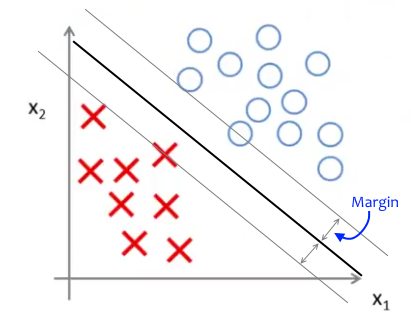
\includegraphics[scale=.75]{billeder/svm-margin}
\caption{Large margin classification.}
\label{fig:svm-margin}
\end{figure}
To maximise the margin, the problem must be treated like a constrained optimisation problem.
The margin is found to be $\gamma = \frac{1}{||w||}$.\\
This margin must be maximised by it is subject to the constrain that $\textbf{w}^T\textbf{x}_{new} + b \geq 1$ for class 1 and $\textbf{w}^T\textbf{x}_new + b \leq -1$ for class 2. Using the sign function the constrain can be defined as.
\begin{equation}
t_n(\textbf{w}^T\textbf{x}_{n} + b) \geq 1
\end{equation}
The problem becomes:
\begin{equation*}
\begin{aligned}
& \underset{w}{\text{ARG MAX}}
& & \gamma = \frac{1}{||w||} \\
& \text{subject to}
& & t_n(\textbf{w}^T\textbf{x}_{n} + b) \geq 1, \text{for all n.}
\end{aligned}
\end{equation*}
This can be solved using lagrange multipliers:
\begin{equation}
\begin{aligned}
& \underset{a}{\text{ARG MAX}}
& & a^* =  \sum a_n - \frac{1}{2}\sum_{n,m=1} a_na_mt_nt_m\bar{x}_n^T\bar{x}_m \\
& \text{subject to}
& & a_n \geq 0, \text{  } \sum^N_{n=1}a_nt_n = 0,
\end{aligned}
\end{equation}
For each new sample $x_{new}$ : $t_{new} = sign( \sum a_nt_nx_nx_{new}+b)$ where $\sum a_nt_nx_n$ can be seen as the weight (w). When $a_n \neq 0$ we have a $x_n$ support vector.\\
\ \\
If there is no solution to the SVM, a neat trick can be used called softmax. A slack variable is added to the contraint so the problem becomes:
\begin{equation*}
\begin{aligned}
& \underset{w}{\text{ARG MAX}}
& & \gamma = \frac{1}{||w||} \\
& \text{subject to}
& & t_n(\textbf{w}^T\textbf{x}_{n} + b) \geq 1-\epsilon,\epsilon\geq 0, \text{for all n.}
\end{aligned}
\end{equation*}
This can also be written as
\begin{equation}
w^* = ARG MIN (||w||^* + C \sum \epsilon_n)
\end{equation}
with C determining the weight of the slack variables and $0\leq a_n \leq C$.

%By solving the optimization problem defined as equation \ref{eq:svm-linear-optimization}, we find the parameters for the linear SVM classifier.
%\begin{equation}
%\min_{\theta}C \sum_{i=1}^{m}
%\left[ y^{(i)}cost_1(\theta^Tx^{(i)})+(1-y^{(i)})cost_0(\theta^Tx^{(i)}) \right]
%+ \frac{1}{2}\sum_{i=1}^{n}\theta^2_j
%\label{eq:svm-linear-optimization}
%\end{equation}
%We must choose the value of the constant $C$. \fxnote{(TODO: what is its effect? Some regularization thing. I think it is: C determines the weight of the slack variables)}
%Figure \ref{fig:svm-cost-function} shows the plot of $cost_0$ and $cost_1$.
%\begin{figure}[H]
%\centering
%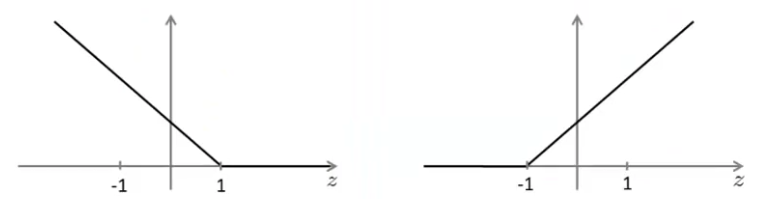
\includegraphics[scale=.75]{billeder/svm-cost-function}
%\caption{Left: $cost_1(\theta^Tx^{(i)})$. Right: $cost_0(\theta^Tx^{(i)})$}
%\label{fig:svm-cost-function}
%\end{figure}
%
%Hypothesis: \fxnote{(TODO: Is this correct? shouldn't it be 1 if} $\theta^Tx \geq 1$ and 0 if $\theta^Tx \leq -1$)
%\begin{equation}
%h = 
%\begin{cases}
%1 & \text{if}\ \theta^Tx \geq 0 \\
%0 & \text{otherwise}
%\end{cases}
%\end{equation}


\subsubsection{Non-linear}
When working with non-linear support vector machine the goal become to find the kernels that separates the data best. These kernels are transformations from one space to another. Three of the most popular kernels are the linear kernel defined as $k( \textbf{x}_n, \textbf{x}_m)= \textbf{x}_n^T\textbf{x}_m$, Gaussian kernels can be defined as equation \ref{eq:gauss1} and polynomial as defined in \ref{eq:polynomial1}.
\begin{equation}
\label{eq:gauss1}
k( \textbf{x}_n, \textbf{x}_m) = e^{-\gamma| \textbf{x}_n -  \textbf{x}_m|^2}
\end{equation}
\begin{equation}
\label{eq:polynomial1}
k( \textbf{x}_n, \textbf{x}_m) = (1+ \textbf{x}_n^T \textbf{x}_m)^{\gamma}
\end{equation}
\begin{figure}[H]
\centering
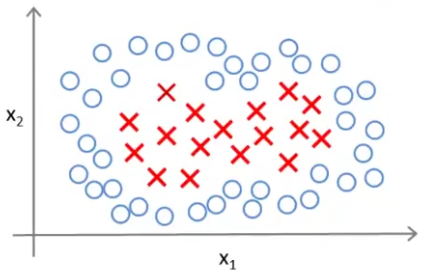
\includegraphics[scale=.75]{billeder/svm-non-linear}
\caption{Example of problem that requires non-linear classification.}
\label{fig:svm-non-linear}
\end{figure}
Observing a problem like that of figure \ref{fig:svm-non-linear} a problem is defined. The optimisation problem from the linear subsection is reformulated to include the kernel functions:
\begin{equation}
\begin{aligned}
& \underset{a}{\text{ARG MAX}}
& & a^* =  \sum a_n - \frac{1}{2}\sum_{n,m=1} a_na_mt_nt_mk( \textbf{x}_n, \textbf{x}_m) \\
& \text{subject to}
& & 0 \leq a_n \leq C, \text{  } \sum^N_{n=1}a_nt_n = 0, \text{for all n.}
\end{aligned}
\end{equation}
and
\begin{equation}
t_{new} = sign(\sum^N_{n=1}a_nt_nk(\textbf{x}_n,\textbf{x}_{new}) + b)
\end{equation}
Taking the Gaussian kernel as an example the decision boundaries will look  like in figure \ref{fig:svm-non-linear2}.
\begin{figure}[H]
\centering
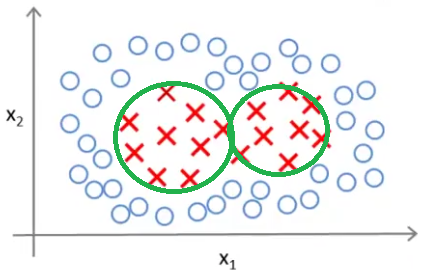
\includegraphics[scale=.75]{billeder/svm-non-linear2}
\caption{Example of classification using SVM and Kernels}
\label{fig:svm-non-linear2}
\end{figure}

%The gaussian kernel function:
%\begin{equation}
%f_i = similarity(x,l^{(i)}) =
%exp\left(-\frac{||x-l^{(i)}||^2}{2\sigma^2}\right)
%\end{equation}
%
%At each training example we will put a landmark:
%\begin{equation}
%\begin{split}
%\text{Given}\ (x^{(1)},y^{(1)}),(x^{(2)},y^{(2)}),\dots,(x^{(m)},y^{(m)}),\\
%\text{choose}\ l^{(1)} = x^{(1)},l^{(2)} = x^{(2)},\dots,l^{(m)} = x^{(m)}
%\end{split}
%\end{equation}
%
%We convert the training data into new feature vectors. For training example $(x^{(i)},y^{(i)})$:
%\begin{equation}
%f^{(i)}=
%\begin{bmatrix}
%f_0^{(i)} \\
%f_1^{(i)} \\
%\vdots \\
%f_m^{(i)}
%\end{bmatrix}
%\end{equation}
% where $f_0^{(i)} = 1$.
%
%The minimization problem now looks like:
%\begin{equation}
%\min_{\theta}C \sum_{i=1}^{m}
%\left[ y^{(i)}cost_1(\theta^Tf^{(i)})+(1-y^{(i)})cost_0(\theta^Tf^{(i)}) \right]
%+ \frac{1}{2}\sum_{i=1}^{m}\theta^2_j
%\end{equation}
%
%A large C gives lower bias and high variance, which means it uses a smaller amount of regularization and is more prone to overfitting. \\
%A small C gives higher bias and low variance, which means it uses a higher amount of regularization and is more prone to underfitting. \\
%A large $\sigma^2$ gives higher bias and lower variance, which means that features $f_i$ varies more smoothly. \\
%A small $\sigma^2$ gives lower bias and higher variance, which means that features $f_i$ varies less smoothly.

In this project the non-linear softmax SVM with Kernels is used. Inputting the features from this project along with a vector \textbf{t} that describes which class the features belong to results in the estimated weights for the SVM classifier. The support vector machine classifier is then used on the speaker recognition test data. When evaluating the test set a 21.68\% error was found. The confusion matrix can be seen in figure \ref{fig:conmatsvm}. 

\begin{figure}[H]
\centering
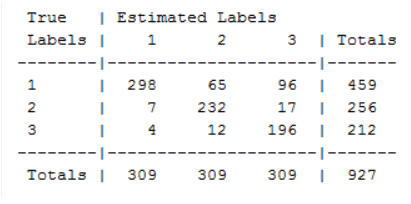
\includegraphics[scale=.75]{billeder/conmatsvm}
\caption{Confusion matrix for the support vector machine }
\label{fig:conmatsvm}
\end{figure}


%------------------------------------------------